\documentclass[aps,jcp,preprint,superscriptaddress]{revtex4}

\usepackage[utf8]{inputenc}
\usepackage{amsmath, amssymb}
\usepackage{tabularx,booktabs,array,dcolumn}
\usepackage{setspace}
\usepackage{vmargin}
\usepackage{graphicx,psfrag,subfigure}
\usepackage{color}
\usepackage[all]{xy}

\usepackage{enumitem}
\usepackage{mdframed}
\usepackage{xcolor}

\sloppy \frenchspacing \clubpenalty=10000 \widowpenalty=10000

\begin{document}

\title{
Melting point convergence with various potentials, effect of the number of atoms, walkers and steps}


\author{}
\affiliation{}
\email{}

\date{\today}

\maketitle

%%%%%%%%%%%%%%%%%%%%%%%%%%%%%%%%%%%%%%%%%%%%%%%%%%%%%%%%%%%%%%%%%%%%%%%%%%
%
% Introduction
%
%%%%%%%%%%%%%%%%%%%%%%%%%%%%%%%%%%%%%%%%%%%%%%%%%%%%%%%%%%%%%%%%%%%%%%%%%%
\section{mW model of water}
\begin{figure}[hbt]
\begin{center}
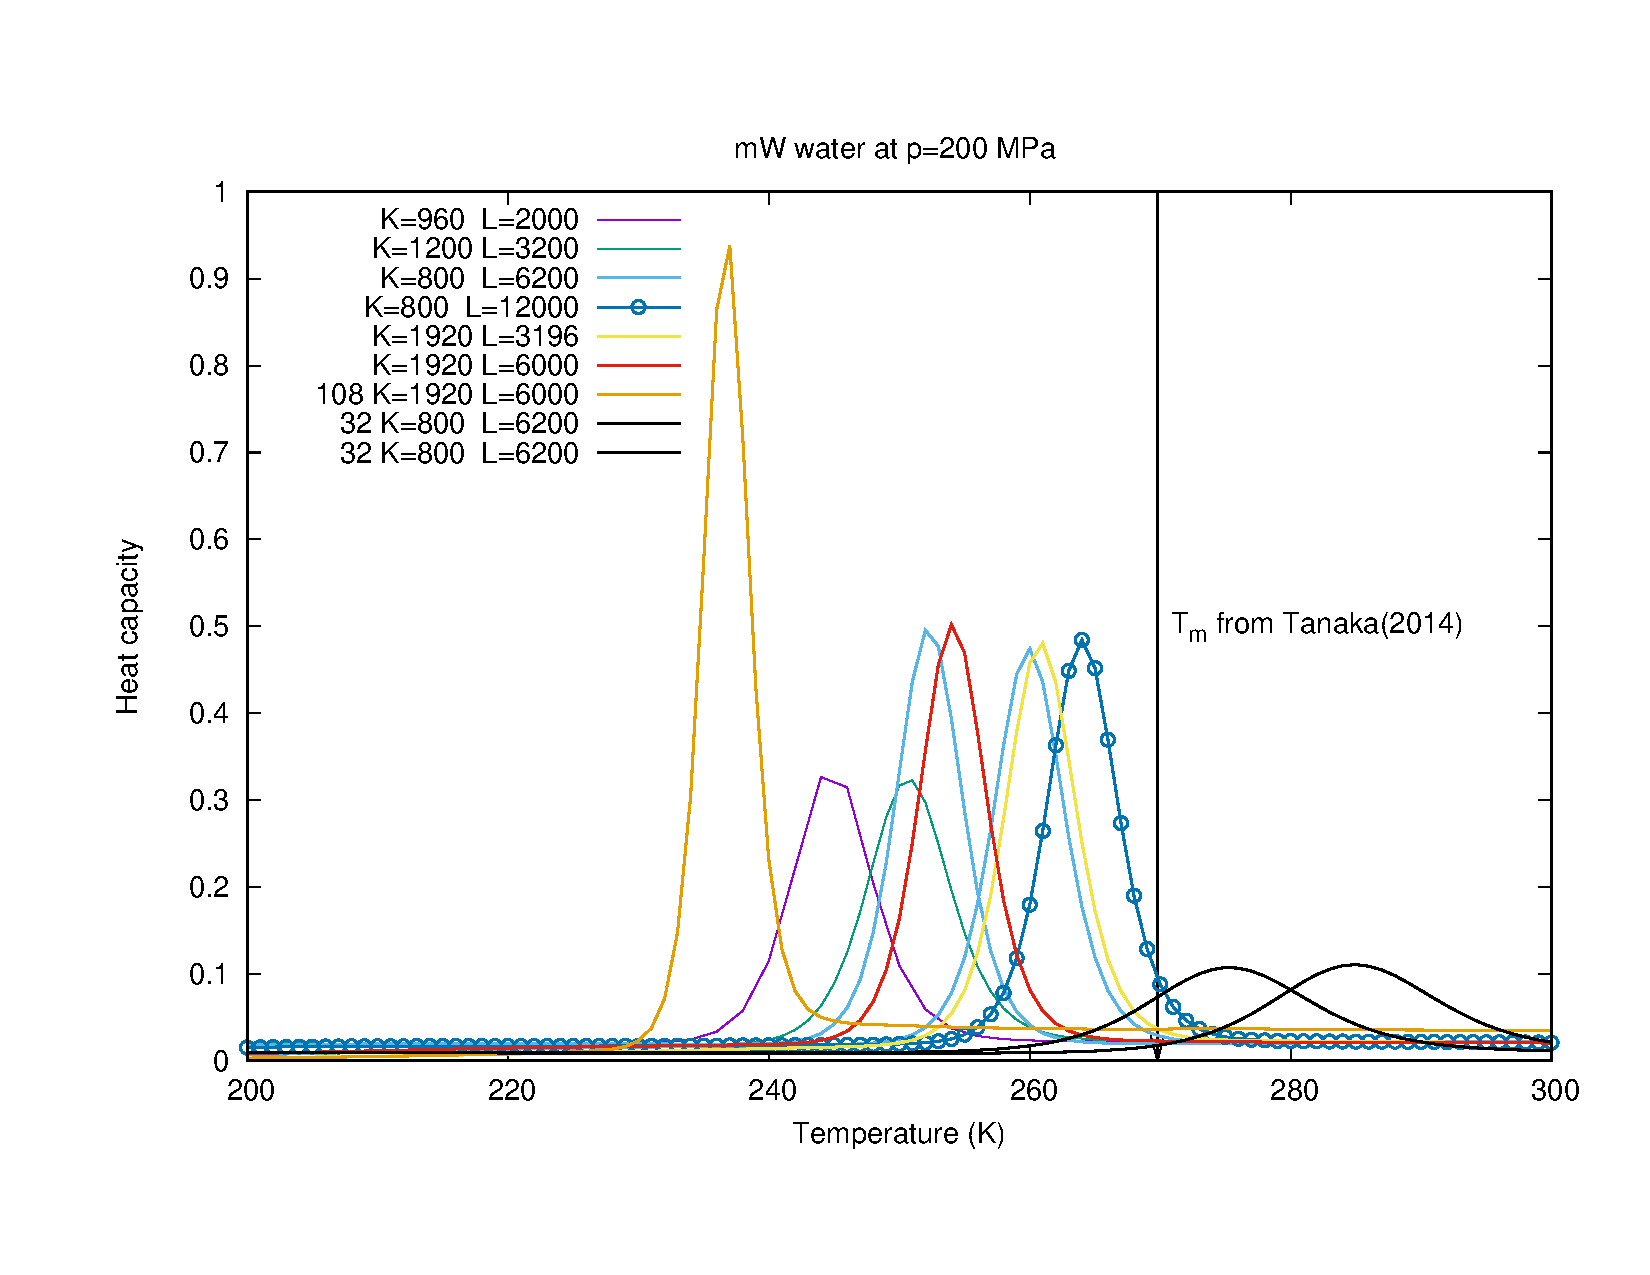
\includegraphics[width=14cm]{mW-fig.pdf}
\end{center}
\vspace{-20pt}
\caption {Predicted melting temperature of the mW model at 200 MPa, for 32, 64 and 128 atoms.}
\label{fig:mW}
\end{figure}


\section{Au EAM model}
\vspace{3cm}
\begin{figure}[hbt]
\begin{center}
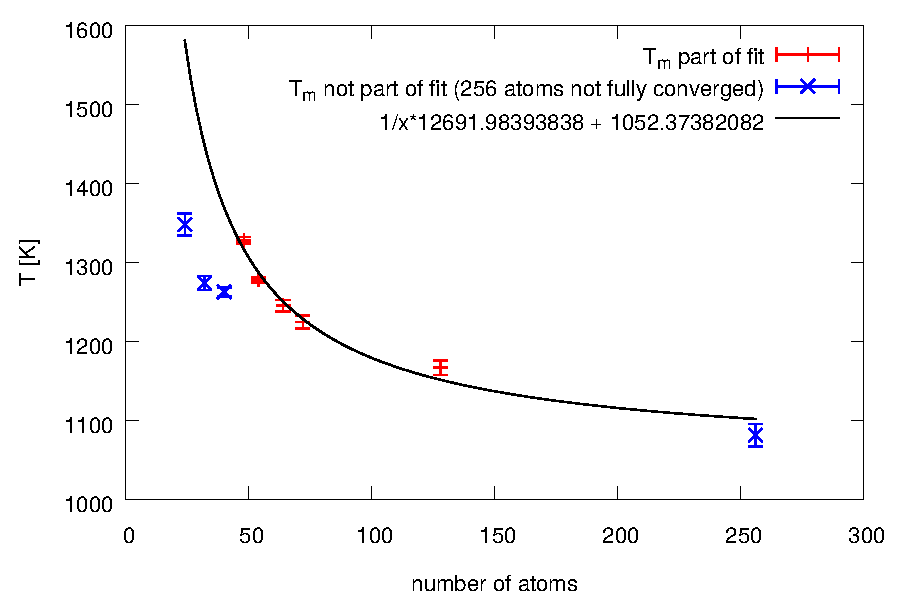
\includegraphics[width=13.1cm]{Au_melting_temperatures_with_fit.pdf}
\end{center}
\vspace{-20pt}
\caption {$T_M$ versus number of atoms. For parameters, see Table \ref{table:Au_parmeters}. Coexistence simulations point towards a melting temperature between $1660$\,K and $1690$\,K.}
\label{fig:mW}
\end{figure}

\begin{figure}[hbt]
\begin{center}
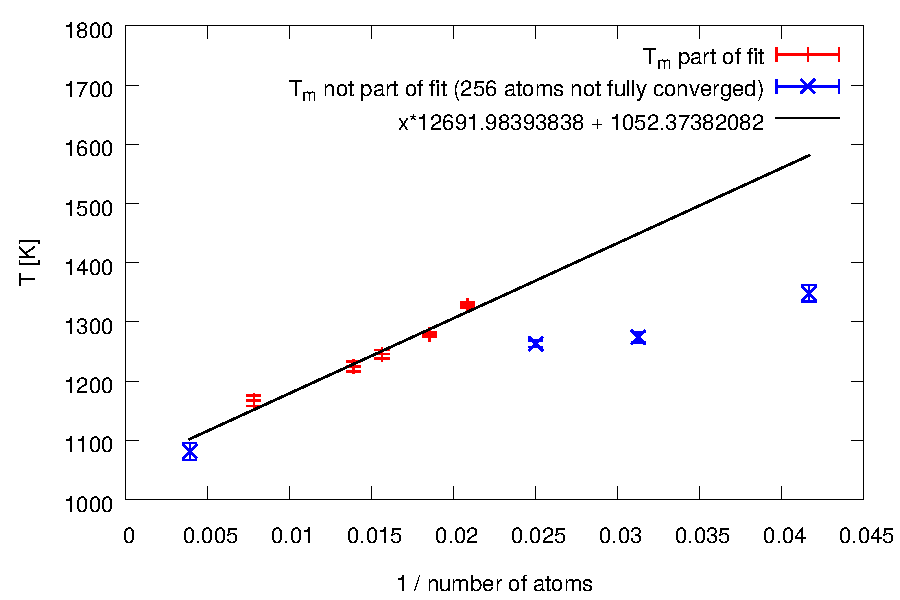
\includegraphics[width=13.1cm]{Au_melting_temperatures_with_fit_1_over_N.pdf}
\end{center}
\vspace{-20pt}
\caption {$T_M$ versus $1/n_{atoms}$. For parameters, see Table \ref{table:Au_parmeters}. Coexistence simulations point towards a melting temperature between $1660$\,K and $1690$\,K.}
\label{fig:mW}
\end{figure}



\begin{center}
\resizebox{13cm}{!} {
  \begin{tabular}{| c | c | c | c | c |}
    \hline
    $n_\text{atoms}$         & $n_\text{cull}$ & $n_\text{walkers}$ & $n_\text{steps}$ & $V_\text{start}$ \\ \hline
    $24$, $32$, $48$, $54$, $72$ &     $8$    &     $1152$    &     $768$   &    $2500$  \\ \hline
    $64$, $128$                  &     $1$    &     $1152$    &     $768$   &   $10000$  \\ \hline
    $256$                        &     $1$    &     $1152$    &    $1536$   &   $10000$  \\
    \hline
    \label{table:Au_parmeters}
  \end{tabular}
}
